\chapter{Learning Analytics}
\section{Cos'è il Learning Analytics}
La delicata e importante tematica della privacy e della sicurezza affrontata nel capitolo precedente influenza fortemente anche il settore
del Learning Analytics.
\begin{wrapfigure}{r}{0.25\textwidth}
    \centering
    
\includegraphics[width=0.25\textwidth]{Immagini/Dragan Gasevic.jpg}
    \caption{Dragan Gasevic}
    \subcaption{Padre di Learning Analytics}
\end{wrapfigure}
Questo particolare ramo emergente dell'educazione si occupa di misurare e analizzare i dati ottenuti dagli studenti e dai loro corsi
di studio, con l'obiettivo di ottimizzare l'esperienza educativa e migliorare non solo i loro risultati, ma anche i metodi di insegnamento. 
\\Grazie alla crescente digitalizzazione e all'adozione di strumenti 
come i Learning Management System (LMS), i social media e i corsi online aperti e massivi (MOOCs), è possibile raccogliere una grande quantità di dati relativi al comportamento degli studenti, 
ai loro risultati e alle interazioni con i materiali didattici. 
\\Il Learning Analytics offre un enorme aiuto a tutti gli stakeholder coinvolti nel processo educativo:
\begin{itemize}
    \item gli studenti possono riflettere sui propri progressi e migliorare il proprio apprendimento attraverso feedback personalizzati e a loro volta dare feedback sui corsi per aiutare i docenti a migliorare i metodi di insegnamento;
    \item i docenti possono adattare i contenuti dei corsi in base ai feedback e ai risultati lasciati dagli studenti e identificare tempestivamente quali tra loro sono in difficoltà;
    \item gli amministratori accademici possono utilizzare i dati per prendere decisioni basate sull'evidenza e sviluppare strategie efficaci per migliorare l'efficienza e la qualità dell'istruzione.
\end{itemize}
Proprio per questo le principali applicazioni del Learning Analytics sono il monitoraggio delle prestazioni individuali, la prevenzione dell'abbandono scolastico,
la personalizzazione dei percorsi educativi e l'analisi delle tecniche di valutazione e dei curricula \cite{wikipedia_learning_analytics}.

\section{Limiti del Learning Analytics}
Nonostante la disponibilità di standard di riferimento per la gestione dei dati di apprendimento su un LRS (Learning Record Store), è ancora difficile raggiungere l'interoperabilità,
ovvero la capacità di due piattaforme differenti di scambiare le informazioni in maniera indipendentemente, senza alcune limitazioni.
\\Questi problemi inducono a:
\begin{itemize}
    \item difficoltà nel collegare le storie di apprendimento di uno studente su diverse piattaforme di apprendimento in un unico percorso immutabile, in modo tale che ogni studente non abbia diverse identità in base alle piattaforme su cui si collega;
    \item difficoltà nel garantire la privacy dei registri degli studenti mantenendo un controllo degli accessi facilitato;
    \item difficoltà nell'integrare sistemi di ricerca e di produzione per migliorare l'apprendimento.
\end{itemize}

\subsection{Collegare le storie di apprendimento }
Sebbene gli studenti spesso passino da una piattaforma di apprendimento di un provider a un'altra, i loro record vengono memorizzati separatamente in LRS distinti e in modo disconnesso. 
Di conseguenza, ogni sistema deve sostenere il costo di ricostruire i dati dell'apprendente da zero anche per casi molto semplici. Nonostante questo potrebbe non rappresentare uno sforzo ripetuto per i principianti, è quasi impossibile determinare se uno studente sia effettivamente un principiante.
\\Questo genera un problema di "\textit{cold start}" nei sistemi di raccomandazione per la formazione, a causa della mancanza di azioni di apprendimento precedenti degli studenti \cite{barnes_stamper_2008}.
\\I sistemi proposti dovrebbero consentire agli studenti di portare con sé i propri dati di apprendimento,
nello stesso modo in cui possono facilmente trasferire i certificati da un'istituzione all'altra. 
\\A tal proposito tornerebbe utile il design del Web 3.0 presentato nel capitolo precedente che permetterebbe a ogni studente di costruirsi un'identità digitale univoca indipendente dal provider di servizi e che consentirebbe di
andare a risolvere il problema di cold start, in quanto non servirebbe più ricostruire ogni volta la storia di apprendimento di uno studente, ma basterebbe andare a leggere la sua identità digitale \cite{ocheja2018connecting}.

\subsection{Privacy, sicurezza e controllo degli accessi}
Questo è un ulteriore problema che si riscontra nel momento in cui si condividono i risultati di apprendimento individuali degli studenti con terze parti. 
\\Sebbene l'analisi dell'apprendimento aiuti a migliorare le prestazioni degli studenti, le loro normative sulla privacy, sostengono che, qualunque siano i guadagni dalle analisi dell'apprendimento, queste devono sempre tener conto al rispetto della privacy e dei diritti.
\\Questo implica che non si potrà andare a violare la privacy dello studente per avere una maggiore efficienza dalle analisi dell'apprendimento,
in quanto il trauma psicologico che potrebbe derivare da una singola violazione della privacy può essere devastante, poiché è possibile rivelare informazioni riservate e dunque sensibili. 
\\I sistemi proposti devono quindi garantire in primis la priorità al rispetto della privacy degli studenti, lasciando a loro il controllo decisionale dei propri dati di apprendimento \cite{ocheja2018connecting}.

\subsection{Integrare i sistemi di ricerca e produzione}
La disponibilità di dati di apprendimento per la ricerca favorisce l'innovazione. 
Nei casi in cui i dati di apprendimento siano raccolti da sistemi di produzione e/o di ricerca, i ricercatori di learning analytics spesso si trovano a dover affrontare il difficile compito di anonimizzare le informazioni personali, con lo scopo di mantenere protetta la privacy degli stakeholder.
\\Facendo così, si ha però un'immensa dispersione di risorse impiegate nel processo di anonimizzazione e inoltre si ha un impatto negativo sui risultati, perchè si va a perderne la loro caratterizzazione e personalizzazione. 
\\Poiché i dati di apprendimento in tempo reale diventano sempre più desiderabili per la ricerca in learning analytics, è cruciale sviluppare nuove idee su come integrare in modo fluido e interoperabile i sistemi di ricerca e di produzione, garantendo al contempo la privacy di tutti gli stakeholder coinvolti \cite{ocheja2018connecting}.

\newpage
\section{Blockchain come soluzione}
Ogni stakeholder deve avere diritti diversi sui dati e metadati, 
di conseguenza, questi devono essere circondati da diversi livelli di accesso degli utenti, ciascuno con permessi specifici e unici,
in modo tale che gli studenti possano avere accesso solamente ai loro dati, gli insegnanti ai dati di tutti i loro studenti, mentre i genitori solo ai dati relativi ai propri figli.
\\La natura di questi diritti e il modo in cui vengono applicati devono essere concordati in modo esplicito e chiaramente comprensibile da tutti, 
inoltre potrebbero essere validi solo per periodi di tempo limitati e vincolati al soddisfacimento di determinate condizioni, in modo tale da garantire un'adeguata anonimizzazione dei dati per rispettare la privacy di ciascun stakeholder.
\\Ha quindi senso archiviare tutti i dati e metadati rilevanti relativi allo studente per le Learning Analytics in un decentralized distributed ledger basato su un sistema Blockchain \cite{Learning_Analytics_Privacy_on_the_Blockchain}.
\\Grazie a questo sistema si potranno andare a soddisfare i seguenti requisiti:
\vspace{1em}
\begin{adjustwidth}{1cm}{0pt}
    \begin{itemize}[itemsep=1ex]
        \item[\textbullet\ \textit{autenticità} $\rightarrow$ ] i "\textit{Data and Metadata About Learning Processes}" (DALP) avranno la prova di essere validi e di essere stati aggiunti da utenti autorizzati;
        \\Questo è molto importante, perchè dire "\textit{Uno studento sostiene di aver preso un 30 all'esame}" non è la stessa cosa di dire "\textit{L'insegnante sostiene che lo studente abbia preso 30}";
        \item[\textbullet\ \textit{integritàtà} $\rightarrow$ ] i dati non potranno essere modificati;
        \item[\textbullet\ \textit{controllo} $\rightarrow$ ] solo gli stakeholder autorizzati avranno il diritto di accedere ai dati, ma solo a quelli che gli corrispondono;
        \item[\textbullet\ \textit{conoscenza} $\rightarrow$ ] verrà sempre tenuta traccia sul registro di chi ha acceduto ai dati e il motivo per cui lo ha fatto;
        \item[\textbullet\ \textit{sicurezza} $\rightarrow$ ] i dati saranno protetti da furti e attacchi informatici, grazie al design della Blockchain.
    \end{itemize}
\end{adjustwidth}
\vspace{1em}
\'E facile notare come la nascita di una piattaforma che necessita questi requisiti sarebbe molto più spontanea, naturale e meno costosa se 
fosse inserita in un ecosistema che la favorisse soddisfandone già a sua volta i requisiti.
\\\'E importante quindi evidenziare ancora una volta l'importanza che avrebbe il passaggio del web da 2.0 a 3.0 e gli innumerevoli vantaggi che ciò comporterebbe.
\\Nei paragrafi che seguiranno vedremo nel dettaglio alcuni esempi tangibili di piattaforme Blockchain-based nell'ambito educativo che sono al momento dispobili sul web.

\newpage
\section{EduCTX}
La più importante piattaforma nel settore educativo basata su Blockchain è EduCTX, sviluppata da un consorzio di università europee sfrutta la Blockchain 2.0 di Ethereum con lo scopo di gestire i crediti e le valutazioni nell'istruzione superiore.
\\In ambito di Learning Analytics è molto importante l'apporto di EduCTX, in quanto permette di raccogliere i certificati e i risultati degli studenti sui quali effettuare successivamente le analisi.
\\Al momento questa piattaforma presenta due versioni, la versione 1.2 sulla quale noi focalizzeremo il nostro interesse in quanto costruita su Blockchain
sfruttando il portale di registrazione MetaMask e la versione 2.0 che invece si basa su Microsoft Azure Active Directory un servizio di gestione d'identità centralizzato basato su cloud.
\begin{figure}[h]
    \centering
    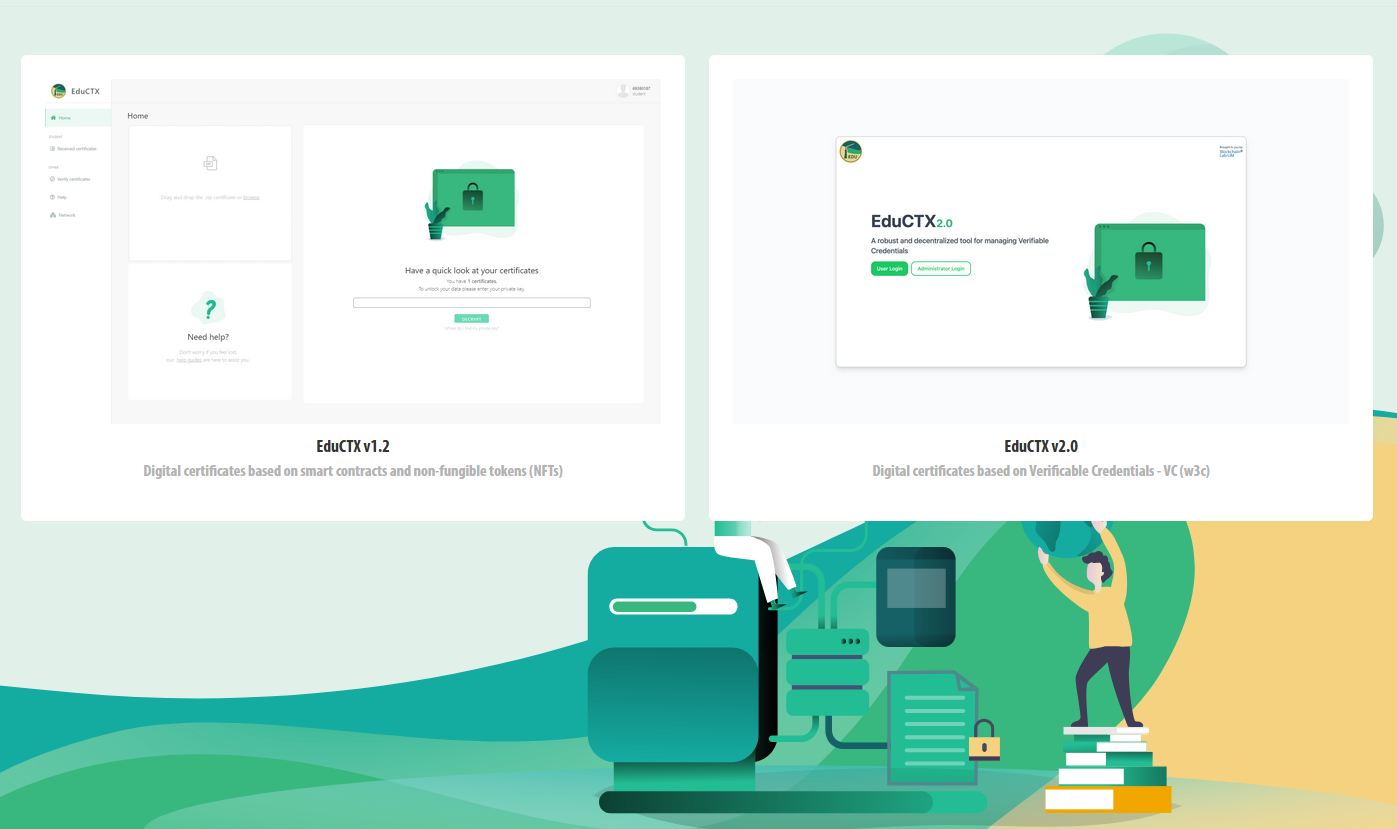
\includegraphics[width=0.85\textwidth]{Immagini/EduCTX.PNG}
    \caption{EduCTX homepage}
\end{figure}

\subsection{Struttura}
La piattaforma EduCTX è concepita per elaborare, gestire e controllare i token ECTX come crediti accademici, basandosi su una rete P2P globalmente distribuita, 
in cui i nodi della rete blockchain sono gli istituti di istruzione superiore (HEI), mentre gli utenti della piattaforma sono studenti e organizzazioni.
\\I token ECTX rappresentano l’equivalente del valore dei crediti ottenuti dagli studenti per i corsi completati.
\\Ogni studente disporrà di un wallet blockchain dedicato sulla piattaforma EduCTX, in cui potrà raccogliere i token ECTX, ossia il valore dei crediti assegnati dall’HEI per i corsi completati. 
\\Ogni volta che uno studente completa un corso, l’HEI di appartenenza trasferirà il numero appropriato di token ECTX al suo indirizzo blockchain. 
\\Le informazioni sul trasferimento vengono archiviate sulla blockchain, 
includendo i seguenti dati: 
\begin{itemize}
    \item il mittente, identificato come l’HEI con il suo nome ufficiale;
    \item il destinatario, presentato in modo anonimo;
    \item il token, valore del credito del corso;
    \item l’ID del corso.
\end{itemize}
Utilizzando il proprio indirizzo blockchain, lo studente, in qualità di destinatario dei token ECTX, può dimostrare globalmente i corsi completati, senza ostacoli amministrativi, di traduzione o linguistici, semplicemente presentando il suo indirizzo blockchain. 
\\Per garantire la sicurezza, agli studenti viene assegnato un indirizzo con firma multipla 2-2 da parte dell’HEI di appartenenza, impedendo loro di trasferire i token ECTX guadagnati verso altri indirizzi. 
\\Il processo di assegnazione dei token ECTX agli studenti e la loro capacità di dimostrarne il possesso sono gestiti tramite un client API blockchain EduCTX facile da usare che rende l’utilizzo della piattaforma il più intuitivo possibile.
\begin{figure}[h]
    \centering
    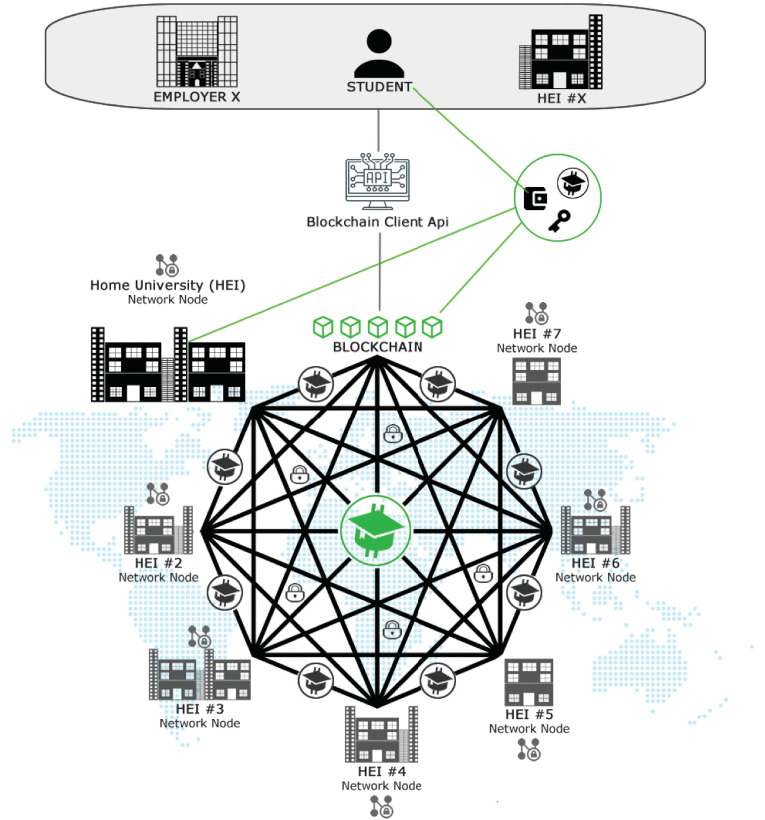
\includegraphics[width=0.65\textwidth]{Immagini/EduCTX_blockchain_structure.jpg}
    \caption{EduCTX struttura blockchain}
\end{figure}

\subsection{Registrazione degli HEI}
Qualsiasi HEI accreditato e i suoi membri potranno entrare a far parte della rete. 
Per aderire, l’HEI dovrà configurare un nodo di rete per mantenere un’infrastruttura globale e una rete sicura. 
Un nodo completamente funzionante trasmette messaggi attraverso la rete, primo passo del processo di transazione che porta alla conferma di un blocco, e quindi alla conferma del trasferimento dei crediti ECTX agli studenti per i corsi completati. 
Il nodo HEI include anche il client blockchain EduCTX principale nel proprio server, con la replica completa del registro blockchain. Questo aumenta la sicurezza, poiché un numero maggiore di nodi rende la rete più sicura.
Gli HEI, e quindi i nodi, non minano le transazioni, poiché la piattaforma blockchain EduCTX è basata sul protocollo di consenso DPoS. Pertanto, non è necessaria alcuna potenza di calcolo da parte del nodo HEI. 
Questo approccio è inoltre appropriato dal punto di vista della sicurezza per la rete EduCTX, poiché peer casuali non possono unirsi alla rete e generare nuovi token ECTX attraverso il mining. 
\\Di conseguenza, la blockchain EduCTX può essere considerata una versione consortile di una blockchain, ovvero una versione specifica di permissioned.
\\Ogni nuovo HEI che si unisce alla rete e viene verificato dagli altri membri HEI, riceve un’assegnazione iniziale di token ECTX e viene invitato a configurare un nodo di rete. 
\\Essendo una blockchain DPoS, ogni membro HEI può registrarsi come delegato nella piattaforma blockchain EduCTX e la comunità HEI vota un delegato che conferma le transazioni e sigilla i blocchi. 
Questo implica che la comunità vota per l’HEI più attivo e continuo nel suo lavoro. 
\\Per garantire una versione permissioned della piattaforma blockchain e una comunità democratica e senza scopo di lucro, la ricompensa per il forging è nulla \cite{EduCTX}.

\subsection{Registrazione degli studenti}
Quando uno studente si immatricola presso un HEI (membro della rete blockchain EduCTX), l'istituto emette un ID studente e genera un nuovo indirizzo blockchain per lo studente, contenente una chiave pubblica e una chiave privata
e anche un nuovo indirizzo blockchain con firma multipla 2-2 utilizzando la propria chiave pubblica e quella appena generata dello studente. 
\\Questo indirizzo con firma multipla, insieme all'ID studente, viene memorizzato nel database dell'HEI.
\\L'HEI trasferisce 0,1 token ECTX all'indirizzo blockchain con firma multipla 2-2 dello studente e, tramite un canale privato, fornisce allo studente le informazioni necessarie per configurare il portafoglio blockchain. 
\\Le informazioni fornite includono:
\begin{itemize}
    \item istruzioni per configurare un portafoglio blockchain EduCTX;
    \item l'indirizzo blockchain dello studente, contenente chiavi pubbliche e private;
    \item la chiave pubblica dell'HEI;
    \item lo script di riscatto (redeem script).
\end{itemize}
Con le informazioni ricevute, lo studente configura il proprio portafoglio blockchain e un singolo indirizzo, utilizzando le chiavi pubbliche e private fornite dall'amministrazione dell'HEI.

\section{Sony Global Education e Blockcerts}
Due importanti menzioni d'onore da fare nell'ambito dell'istruzione basata su Blockchain sono Sony Global Education e Blockcerts.
\\La prima è a tutti gli effetti una piattaforma di Learning Analytics basata su una Blockchain permissioned, sviluppata per l'appunto da Sony, con l'obiettivo di raccogliere i dati 
sull'appredimento dei giovanissimi andando a migliorarne il loro percorso di apprendimento, con un focus particolare sullo sviluppo della loro creatività.
\begin{figure}[h]
    \centering
    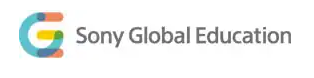
\includegraphics[width=0.65\textwidth]{Immagini/Sony_Global_Education_logo.PNG}
    \caption{Sony Global Education Logo}
\end{figure}
\\Blockcerts è invece una piattaforma sviluppata dal MIT Media Lab in collaborazione con Learning Machine. 
\\Questa piattaforma è sullo stampo di EduCTX,
infatti può emettere certificati, o inoltre, può permettere agli studenti di archiviare e verificare i loro certificati accademici, attestati professionali e altre credenziali.
\\In questo modo chiuque può verificare l'autenticità di un certificato senza dover contattare l'istituzione che lo ha rilasciato.
\\Questa piattaforma è basata su una Blockchain permissionless ed inizialmente è stata progettata per ancorare i certificati sulla blockchain di Bitcoin, 
ma successivamente ha iniziato a supportare Ethereum in modo tale da poter sfruttare gli Smart Contracts.
\begin{figure}[h]
    \centering
    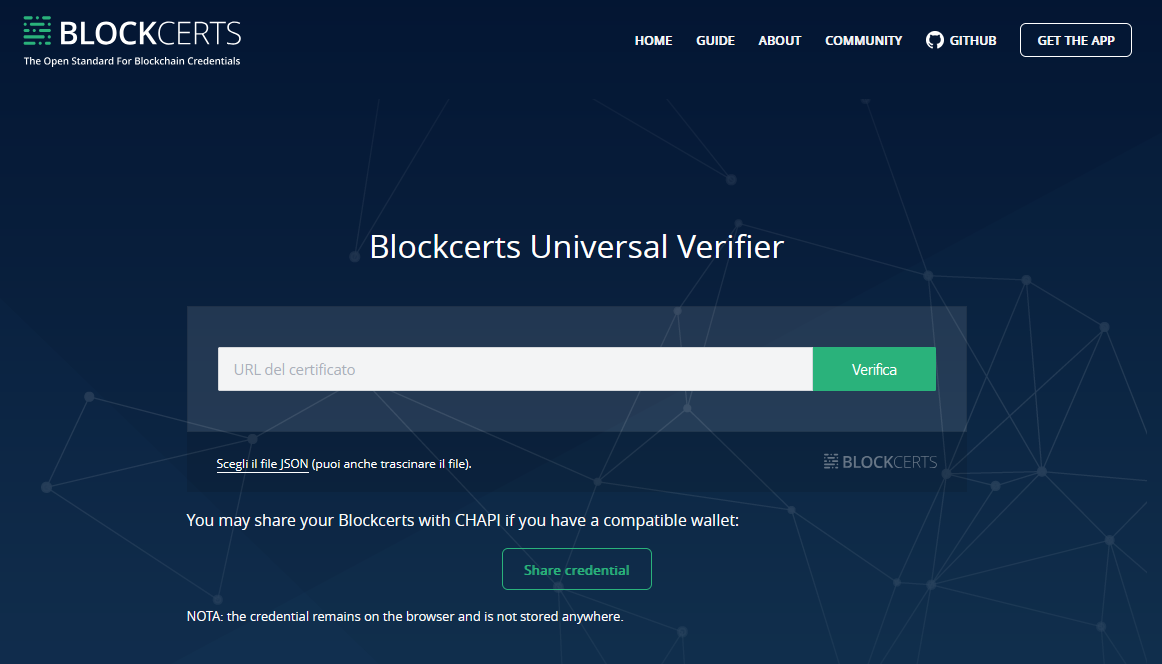
\includegraphics[width=0.65\textwidth]{Immagini/Blockcerts_homepage.PNG}
    \caption{Blockcerts homepage}
\end{figure}
\\Da fine 2019 Blockcerts è stata adottata anche dall'università di Padova, che ha iniziato a rilasciare i certificati di laurea in formato digitale scaricabli dalla piattaforma Bestr.
